% Adopted endpoint orientation. Generated from the verified full finite table.
% Original raster remains unchanged. Outcome probabilities apply to each displayed alternative.
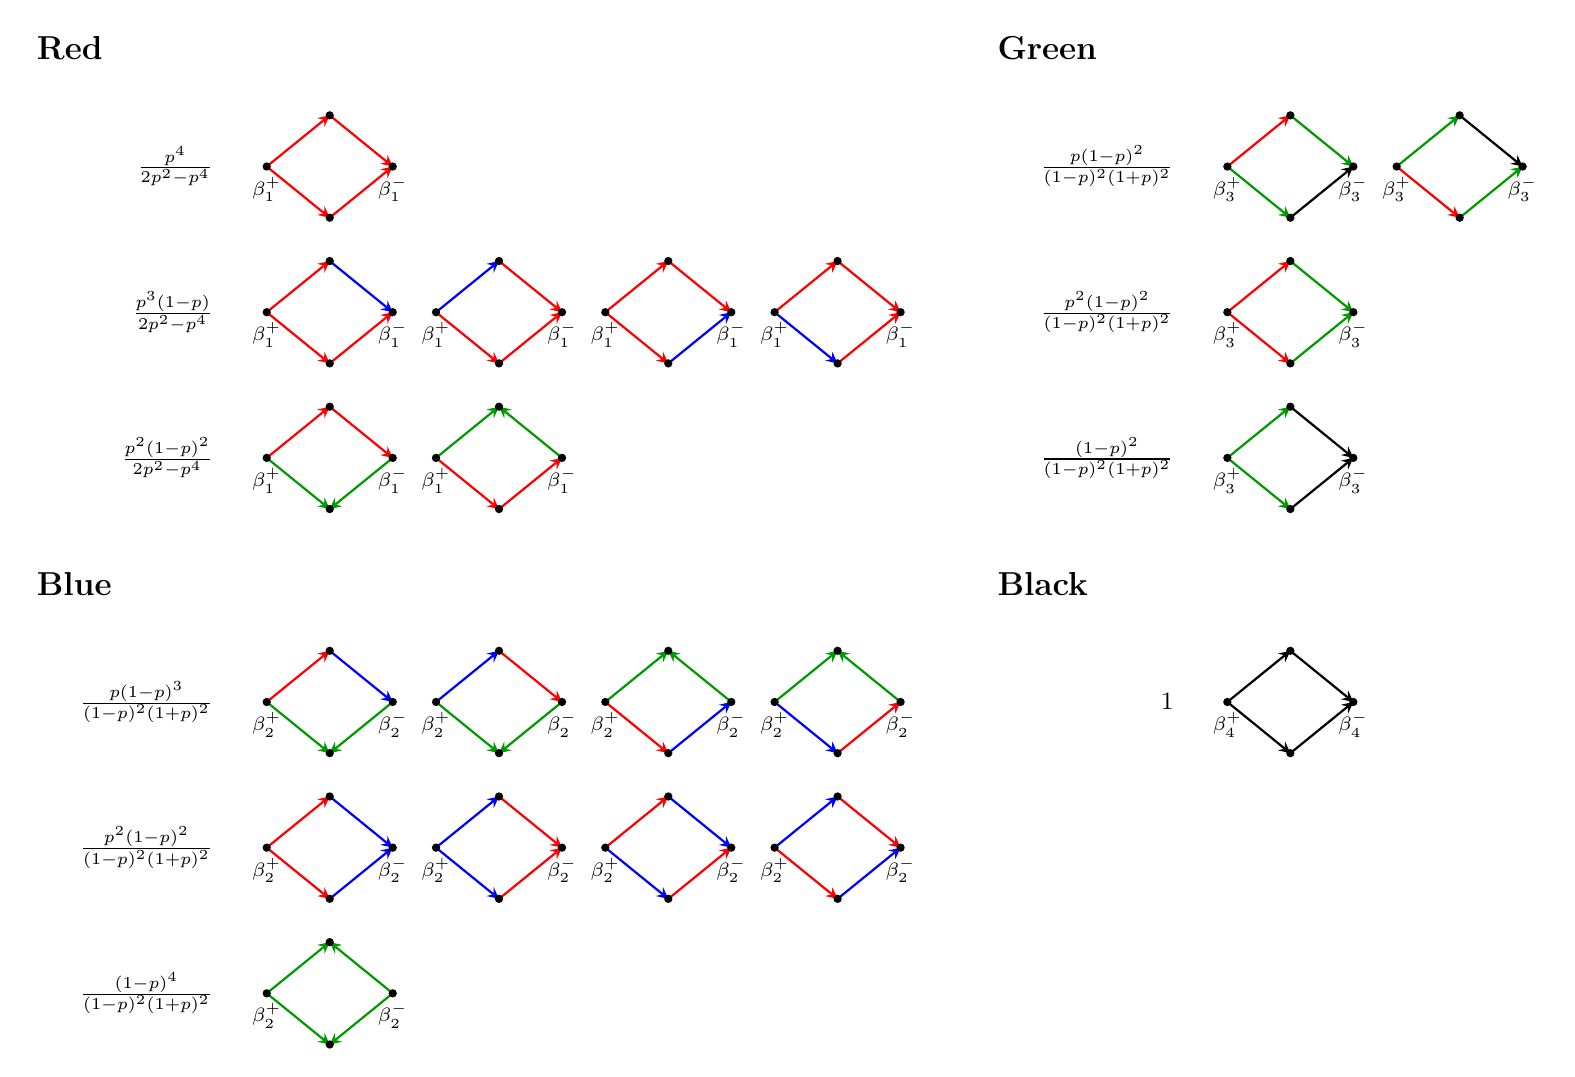
\begin{tikzpicture}[>=stealth, line width=0.8pt, font=\small]
\node[anchor=west,font=\bfseries\large] at (0,0.5) {Red};
\node[anchor=east] at (2.5,-1.0) {$ \frac{p^4}{2p^2-p^4} $};
\draw[->,red] (3.05, -1.0) -- (3.8499999999999996, -0.35);
\draw[->,red] (3.8499999999999996, -0.35) -- (4.65, -1.0);
\draw[->,red] (3.05, -1.0) -- (3.8499999999999996, -1.65);
\draw[->,red] (3.8499999999999996, -1.65) -- (4.65, -1.0);
\fill (3.05, -1.0) circle (1.5pt);
\fill (3.8499999999999996, -0.35) circle (1.5pt);
\fill (4.65, -1.0) circle (1.5pt);
\fill (3.8499999999999996, -1.65) circle (1.5pt);
\node[below,font=\scriptsize] at (3.05, -1.0) {$\beta_{1}^+$};
\node[below,font=\scriptsize] at (4.65, -1.0) {$\beta_{1}^-$};
\node[anchor=east] at (2.5,-2.85) {$ \frac{p^3(1-p)}{2p^2-p^4} $};
\draw[->,red] (3.05, -2.85) -- (3.8499999999999996, -2.2);
\draw[->,blue] (3.8499999999999996, -2.2) -- (4.65, -2.85);
\draw[->,red] (3.05, -2.85) -- (3.8499999999999996, -3.5);
\draw[->,red] (3.8499999999999996, -3.5) -- (4.65, -2.85);
\fill (3.05, -2.85) circle (1.5pt);
\fill (3.8499999999999996, -2.2) circle (1.5pt);
\fill (4.65, -2.85) circle (1.5pt);
\fill (3.8499999999999996, -3.5) circle (1.5pt);
\node[below,font=\scriptsize] at (3.05, -2.85) {$\beta_{1}^+$};
\node[below,font=\scriptsize] at (4.65, -2.85) {$\beta_{1}^-$};
\draw[->,blue] (5.199999999999999, -2.85) -- (5.999999999999999, -2.2);
\draw[->,red] (5.999999999999999, -2.2) -- (6.799999999999999, -2.85);
\draw[->,red] (5.199999999999999, -2.85) -- (5.999999999999999, -3.5);
\draw[->,red] (5.999999999999999, -3.5) -- (6.799999999999999, -2.85);
\fill (5.199999999999999, -2.85) circle (1.5pt);
\fill (5.999999999999999, -2.2) circle (1.5pt);
\fill (6.799999999999999, -2.85) circle (1.5pt);
\fill (5.999999999999999, -3.5) circle (1.5pt);
\node[below,font=\scriptsize] at (5.199999999999999, -2.85) {$\beta_{1}^+$};
\node[below,font=\scriptsize] at (6.799999999999999, -2.85) {$\beta_{1}^-$};
\draw[->,red] (7.35, -2.85) -- (8.15, -2.2);
\draw[->,red] (8.15, -2.2) -- (8.95, -2.85);
\draw[->,red] (7.35, -2.85) -- (8.15, -3.5);
\draw[->,blue] (8.15, -3.5) -- (8.95, -2.85);
\fill (7.35, -2.85) circle (1.5pt);
\fill (8.15, -2.2) circle (1.5pt);
\fill (8.95, -2.85) circle (1.5pt);
\fill (8.15, -3.5) circle (1.5pt);
\node[below,font=\scriptsize] at (7.35, -2.85) {$\beta_{1}^+$};
\node[below,font=\scriptsize] at (8.95, -2.85) {$\beta_{1}^-$};
\draw[->,red] (9.5, -2.85) -- (10.3, -2.2);
\draw[->,red] (10.3, -2.2) -- (11.1, -2.85);
\draw[->,blue] (9.5, -2.85) -- (10.3, -3.5);
\draw[->,red] (10.3, -3.5) -- (11.1, -2.85);
\fill (9.5, -2.85) circle (1.5pt);
\fill (10.3, -2.2) circle (1.5pt);
\fill (11.1, -2.85) circle (1.5pt);
\fill (10.3, -3.5) circle (1.5pt);
\node[below,font=\scriptsize] at (9.5, -2.85) {$\beta_{1}^+$};
\node[below,font=\scriptsize] at (11.1, -2.85) {$\beta_{1}^-$};
\node[anchor=east] at (2.5,-4.7) {$ \frac{p^2(1-p)^2}{2p^2-p^4} $};
\draw[->,red] (3.05, -4.7) -- (3.8499999999999996, -4.05);
\draw[->,red] (3.8499999999999996, -4.05) -- (4.65, -4.7);
\draw[->,green!60!black] (3.05, -4.7) -- (3.8499999999999996, -5.3500000000000005);
\draw[->,green!60!black] (4.65, -4.7) -- (3.8499999999999996, -5.3500000000000005);
\fill (3.05, -4.7) circle (1.5pt);
\fill (3.8499999999999996, -4.05) circle (1.5pt);
\fill (4.65, -4.7) circle (1.5pt);
\fill (3.8499999999999996, -5.3500000000000005) circle (1.5pt);
\node[below,font=\scriptsize] at (3.05, -4.7) {$\beta_{1}^+$};
\node[below,font=\scriptsize] at (4.65, -4.7) {$\beta_{1}^-$};
\draw[->,green!60!black] (5.199999999999999, -4.7) -- (5.999999999999999, -4.05);
\draw[->,green!60!black] (6.799999999999999, -4.7) -- (5.999999999999999, -4.05);
\draw[->,red] (5.199999999999999, -4.7) -- (5.999999999999999, -5.3500000000000005);
\draw[->,red] (5.999999999999999, -5.3500000000000005) -- (6.799999999999999, -4.7);
\fill (5.199999999999999, -4.7) circle (1.5pt);
\fill (5.999999999999999, -4.05) circle (1.5pt);
\fill (6.799999999999999, -4.7) circle (1.5pt);
\fill (5.999999999999999, -5.3500000000000005) circle (1.5pt);
\node[below,font=\scriptsize] at (5.199999999999999, -4.7) {$\beta_{1}^+$};
\node[below,font=\scriptsize] at (6.799999999999999, -4.7) {$\beta_{1}^-$};
\node[anchor=west,font=\bfseries\large] at (0,-6.3) {Blue};
\node[anchor=east] at (2.5,-7.8) {$ \frac{p(1-p)^3}{(1-p)^2(1+p)^2} $};
\draw[->,red] (3.05, -7.8) -- (3.8499999999999996, -7.1499999999999995);
\draw[->,blue] (3.8499999999999996, -7.1499999999999995) -- (4.65, -7.8);
\draw[->,green!60!black] (3.05, -7.8) -- (3.8499999999999996, -8.45);
\draw[->,green!60!black] (4.65, -7.8) -- (3.8499999999999996, -8.45);
\fill (3.05, -7.8) circle (1.5pt);
\fill (3.8499999999999996, -7.1499999999999995) circle (1.5pt);
\fill (4.65, -7.8) circle (1.5pt);
\fill (3.8499999999999996, -8.45) circle (1.5pt);
\node[below,font=\scriptsize] at (3.05, -7.8) {$\beta_{2}^+$};
\node[below,font=\scriptsize] at (4.65, -7.8) {$\beta_{2}^-$};
\draw[->,blue] (5.199999999999999, -7.8) -- (5.999999999999999, -7.1499999999999995);
\draw[->,red] (5.999999999999999, -7.1499999999999995) -- (6.799999999999999, -7.8);
\draw[->,green!60!black] (5.199999999999999, -7.8) -- (5.999999999999999, -8.45);
\draw[->,green!60!black] (6.799999999999999, -7.8) -- (5.999999999999999, -8.45);
\fill (5.199999999999999, -7.8) circle (1.5pt);
\fill (5.999999999999999, -7.1499999999999995) circle (1.5pt);
\fill (6.799999999999999, -7.8) circle (1.5pt);
\fill (5.999999999999999, -8.45) circle (1.5pt);
\node[below,font=\scriptsize] at (5.199999999999999, -7.8) {$\beta_{2}^+$};
\node[below,font=\scriptsize] at (6.799999999999999, -7.8) {$\beta_{2}^-$};
\draw[->,green!60!black] (7.35, -7.8) -- (8.15, -7.1499999999999995);
\draw[->,green!60!black] (8.95, -7.8) -- (8.15, -7.1499999999999995);
\draw[->,red] (7.35, -7.8) -- (8.15, -8.45);
\draw[->,blue] (8.15, -8.45) -- (8.95, -7.8);
\fill (7.35, -7.8) circle (1.5pt);
\fill (8.15, -7.1499999999999995) circle (1.5pt);
\fill (8.95, -7.8) circle (1.5pt);
\fill (8.15, -8.45) circle (1.5pt);
\node[below,font=\scriptsize] at (7.35, -7.8) {$\beta_{2}^+$};
\node[below,font=\scriptsize] at (8.95, -7.8) {$\beta_{2}^-$};
\draw[->,green!60!black] (9.5, -7.8) -- (10.3, -7.1499999999999995);
\draw[->,green!60!black] (11.1, -7.8) -- (10.3, -7.1499999999999995);
\draw[->,blue] (9.5, -7.8) -- (10.3, -8.45);
\draw[->,red] (10.3, -8.45) -- (11.1, -7.8);
\fill (9.5, -7.8) circle (1.5pt);
\fill (10.3, -7.1499999999999995) circle (1.5pt);
\fill (11.1, -7.8) circle (1.5pt);
\fill (10.3, -8.45) circle (1.5pt);
\node[below,font=\scriptsize] at (9.5, -7.8) {$\beta_{2}^+$};
\node[below,font=\scriptsize] at (11.1, -7.8) {$\beta_{2}^-$};
\node[anchor=east] at (2.5,-9.65) {$ \frac{p^2(1-p)^2}{(1-p)^2(1+p)^2} $};
\draw[->,red] (3.05, -9.65) -- (3.8499999999999996, -9.0);
\draw[->,blue] (3.8499999999999996, -9.0) -- (4.65, -9.65);
\draw[->,red] (3.05, -9.65) -- (3.8499999999999996, -10.3);
\draw[->,blue] (3.8499999999999996, -10.3) -- (4.65, -9.65);
\fill (3.05, -9.65) circle (1.5pt);
\fill (3.8499999999999996, -9.0) circle (1.5pt);
\fill (4.65, -9.65) circle (1.5pt);
\fill (3.8499999999999996, -10.3) circle (1.5pt);
\node[below,font=\scriptsize] at (3.05, -9.65) {$\beta_{2}^+$};
\node[below,font=\scriptsize] at (4.65, -9.65) {$\beta_{2}^-$};
\draw[->,blue] (5.199999999999999, -9.65) -- (5.999999999999999, -9.0);
\draw[->,red] (5.999999999999999, -9.0) -- (6.799999999999999, -9.65);
\draw[->,blue] (5.199999999999999, -9.65) -- (5.999999999999999, -10.3);
\draw[->,red] (5.999999999999999, -10.3) -- (6.799999999999999, -9.65);
\fill (5.199999999999999, -9.65) circle (1.5pt);
\fill (5.999999999999999, -9.0) circle (1.5pt);
\fill (6.799999999999999, -9.65) circle (1.5pt);
\fill (5.999999999999999, -10.3) circle (1.5pt);
\node[below,font=\scriptsize] at (5.199999999999999, -9.65) {$\beta_{2}^+$};
\node[below,font=\scriptsize] at (6.799999999999999, -9.65) {$\beta_{2}^-$};
\draw[->,red] (7.35, -9.65) -- (8.15, -9.0);
\draw[->,blue] (8.15, -9.0) -- (8.95, -9.65);
\draw[->,blue] (7.35, -9.65) -- (8.15, -10.3);
\draw[->,red] (8.15, -10.3) -- (8.95, -9.65);
\fill (7.35, -9.65) circle (1.5pt);
\fill (8.15, -9.0) circle (1.5pt);
\fill (8.95, -9.65) circle (1.5pt);
\fill (8.15, -10.3) circle (1.5pt);
\node[below,font=\scriptsize] at (7.35, -9.65) {$\beta_{2}^+$};
\node[below,font=\scriptsize] at (8.95, -9.65) {$\beta_{2}^-$};
\draw[->,blue] (9.5, -9.65) -- (10.3, -9.0);
\draw[->,red] (10.3, -9.0) -- (11.1, -9.65);
\draw[->,red] (9.5, -9.65) -- (10.3, -10.3);
\draw[->,blue] (10.3, -10.3) -- (11.1, -9.65);
\fill (9.5, -9.65) circle (1.5pt);
\fill (10.3, -9.0) circle (1.5pt);
\fill (11.1, -9.65) circle (1.5pt);
\fill (10.3, -10.3) circle (1.5pt);
\node[below,font=\scriptsize] at (9.5, -9.65) {$\beta_{2}^+$};
\node[below,font=\scriptsize] at (11.1, -9.65) {$\beta_{2}^-$};
\node[anchor=east] at (2.5,-11.5) {$ \frac{(1-p)^4}{(1-p)^2(1+p)^2} $};
\draw[->,green!60!black] (3.05, -11.5) -- (3.8499999999999996, -10.85);
\draw[->,green!60!black] (4.65, -11.5) -- (3.8499999999999996, -10.85);
\draw[->,green!60!black] (3.05, -11.5) -- (3.8499999999999996, -12.15);
\draw[->,green!60!black] (4.65, -11.5) -- (3.8499999999999996, -12.15);
\fill (3.05, -11.5) circle (1.5pt);
\fill (3.8499999999999996, -10.85) circle (1.5pt);
\fill (4.65, -11.5) circle (1.5pt);
\fill (3.8499999999999996, -12.15) circle (1.5pt);
\node[below,font=\scriptsize] at (3.05, -11.5) {$\beta_{2}^+$};
\node[below,font=\scriptsize] at (4.65, -11.5) {$\beta_{2}^-$};
\node[anchor=west,font=\bfseries\large] at (12.2,0.5) {Green};
\node[anchor=east] at (14.7,-1.0) {$ \frac{p(1-p)^2}{(1-p)^2(1+p)^2} $};
\draw[->,red] (15.25, -1.0) -- (16.05, -0.35);
\draw[->,green!60!black] (16.05, -0.35) -- (16.85, -1.0);
\draw[->,green!60!black] (15.25, -1.0) -- (16.05, -1.65);
\draw[->,black] (16.05, -1.65) -- (16.85, -1.0);
\fill (15.25, -1.0) circle (1.5pt);
\fill (16.05, -0.35) circle (1.5pt);
\fill (16.85, -1.0) circle (1.5pt);
\fill (16.05, -1.65) circle (1.5pt);
\node[below,font=\scriptsize] at (15.25, -1.0) {$\beta_{3}^+$};
\node[below,font=\scriptsize] at (16.85, -1.0) {$\beta_{3}^-$};
\draw[->,green!60!black] (17.4, -1.0) -- (18.2, -0.35);
\draw[->,black] (18.2, -0.35) -- (19.0, -1.0);
\draw[->,red] (17.4, -1.0) -- (18.2, -1.65);
\draw[->,green!60!black] (18.2, -1.65) -- (19.0, -1.0);
\fill (17.4, -1.0) circle (1.5pt);
\fill (18.2, -0.35) circle (1.5pt);
\fill (19.0, -1.0) circle (1.5pt);
\fill (18.2, -1.65) circle (1.5pt);
\node[below,font=\scriptsize] at (17.4, -1.0) {$\beta_{3}^+$};
\node[below,font=\scriptsize] at (19.0, -1.0) {$\beta_{3}^-$};
\node[anchor=east] at (14.7,-2.85) {$ \frac{p^2(1-p)^2}{(1-p)^2(1+p)^2} $};
\draw[->,red] (15.25, -2.85) -- (16.05, -2.2);
\draw[->,green!60!black] (16.05, -2.2) -- (16.85, -2.85);
\draw[->,red] (15.25, -2.85) -- (16.05, -3.5);
\draw[->,green!60!black] (16.05, -3.5) -- (16.85, -2.85);
\fill (15.25, -2.85) circle (1.5pt);
\fill (16.05, -2.2) circle (1.5pt);
\fill (16.85, -2.85) circle (1.5pt);
\fill (16.05, -3.5) circle (1.5pt);
\node[below,font=\scriptsize] at (15.25, -2.85) {$\beta_{3}^+$};
\node[below,font=\scriptsize] at (16.85, -2.85) {$\beta_{3}^-$};
\node[anchor=east] at (14.7,-4.7) {$ \frac{(1-p)^2}{(1-p)^2(1+p)^2} $};
\draw[->,green!60!black] (15.25, -4.7) -- (16.05, -4.05);
\draw[->,black] (16.05, -4.05) -- (16.85, -4.7);
\draw[->,green!60!black] (15.25, -4.7) -- (16.05, -5.3500000000000005);
\draw[->,black] (16.05, -5.3500000000000005) -- (16.85, -4.7);
\fill (15.25, -4.7) circle (1.5pt);
\fill (16.05, -4.05) circle (1.5pt);
\fill (16.85, -4.7) circle (1.5pt);
\fill (16.05, -5.3500000000000005) circle (1.5pt);
\node[below,font=\scriptsize] at (15.25, -4.7) {$\beta_{3}^+$};
\node[below,font=\scriptsize] at (16.85, -4.7) {$\beta_{3}^-$};
\node[anchor=west,font=\bfseries\large] at (12.2,-6.3) {Black};
\node[anchor=east] at (14.7,-7.8) {$ 1 $};
\draw[->,black] (15.25, -7.8) -- (16.05, -7.1499999999999995);
\draw[->,black] (16.05, -7.1499999999999995) -- (16.85, -7.8);
\draw[->,black] (15.25, -7.8) -- (16.05, -8.45);
\draw[->,black] (16.05, -8.45) -- (16.85, -7.8);
\fill (15.25, -7.8) circle (1.5pt);
\fill (16.05, -7.1499999999999995) circle (1.5pt);
\fill (16.85, -7.8) circle (1.5pt);
\fill (16.05, -8.45) circle (1.5pt);
\node[below,font=\scriptsize] at (15.25, -7.8) {$\beta_{4}^+$};
\node[below,font=\scriptsize] at (16.85, -7.8) {$\beta_{4}^-$};
\end{tikzpicture}
